\subsection{Results for Speed}
%\label{subsec:speed_results}
%\vspace{10pt}

Figure~\ref{fig:var_speed.png} represents the $p$-values for the Mann-Whitney $U$-test on actual and predicted values across k-fold validation datasets for the speed in the k-fold testing datasets using different RNN models, and forecasting times. Darker colors in grayscale represent a higher $p$-value in a range from $0$ to $1$. The values on the secondary diagonal are all equal to $1$ and black beacuse each model is equal to itself.

\begin{figure}[!ht]
	\centering
	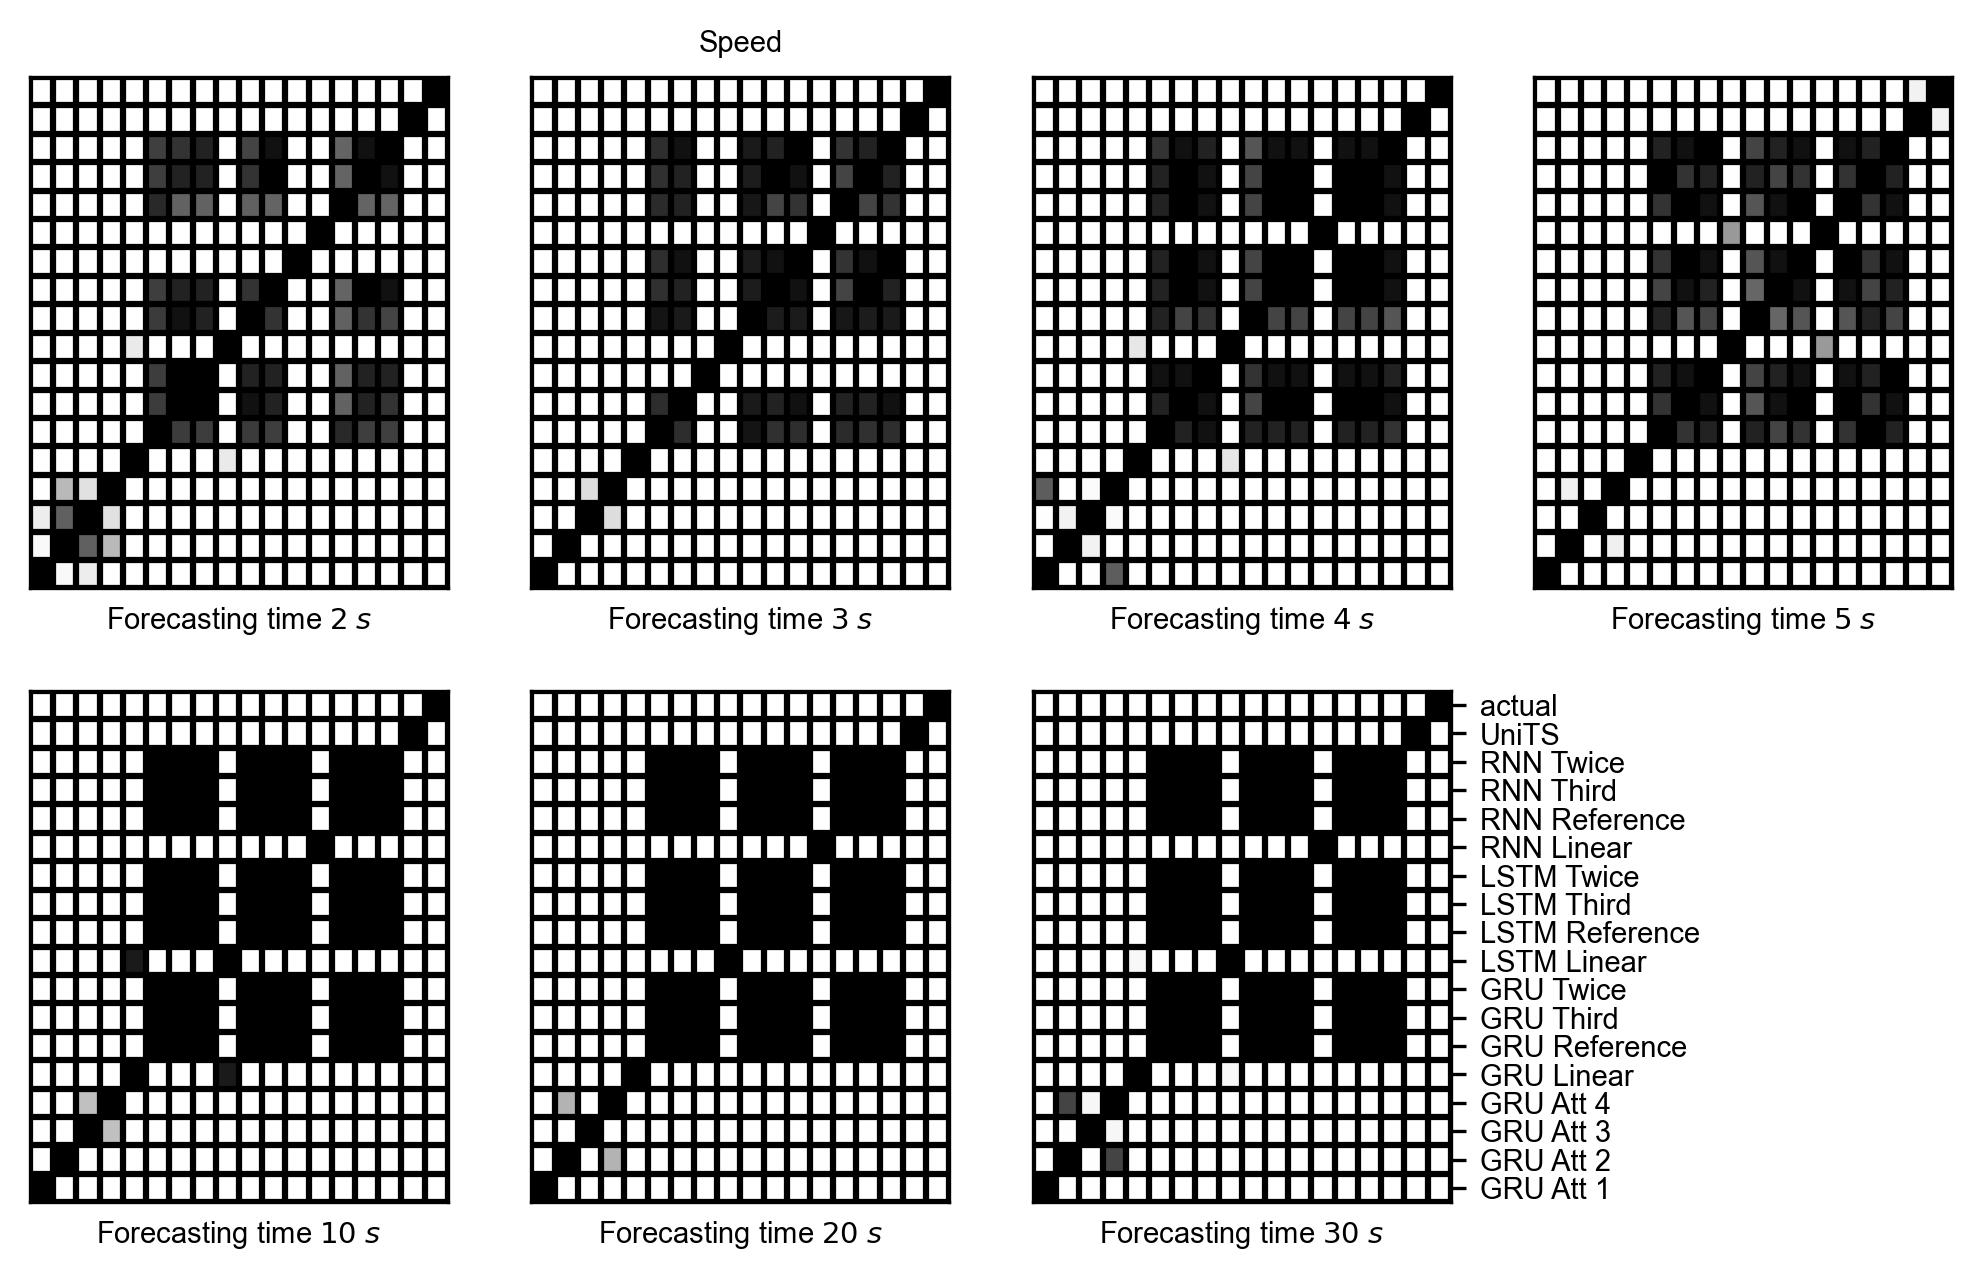
\includegraphics[width = 0.99 \linewidth]{var_speed.png.pdf}
	\caption{The $p$-values for the Mann-Whitney $U$-test on actual and predicted values across k-fold validation datasets for the speed in the k-fold testing datasets using different RNN models, and forecasting times. Darker colors in grayscale represent a higher $p$-value in a range from $0$ to $1$. The values on the secondary diagonal are all equal to $1$ and black beacuse each model is equal to itself.}
	\label{fig:var_speed.png}
\end{figure}

The average $R^{2}$ (\%), with standard deviation in brackets, across k-fold validation datasets for the speed estimated on the k-fold testing datasets by different RNN models, and forecasting times is listed in Table~\ref{tab:best_speed_R2}.

\begin{table}[!ht]
	\centering
	\resizebox{\linewidth}{!}{
		\begin{tabular}{|c|c|c|c|c|c|c|c|}
			\hline
			Model & $2$ $s$ & $3$ $s$ & $4$ $s$ & $5$ $s$ & $10$ $s$ & $20$ $s$ & $30$ $s$ \\ \hline
			\multirow{2}{*}{LSTM Linear} & $\mathbf{94.39\%}$ & $89.11\%$ & $83.69\%$ & $78.54\%$ & $62.8\%$ & $54.98\%$ & $51.44\%$ \\
			 & \textbf{(}$\mathbf{0.63\%}$\textbf{)} & ($1.3\%$) & ($1.83\%$) & ($2.27\%$) & ($3.95\%$) & ($4.2\%$) & ($4.16\%$) \\ \hline
			\multirow{2}{*}{UniTS} & $93.45\%$ & $\mathbf{90.5\%}$ & $\mathbf{87.48\%}$ & $\mathbf{84.54\%}$ & $\mathbf{72.89\%}$ & $\mathbf{61.53\%}$ & $\mathbf{56.21\%}$ \\
			 & ($0.64\%$) & \textbf{(}$\mathbf{0.92\%}$\textbf{)} & \textbf{(}$\mathbf{1.21\%}$\textbf{)} & \textbf{(}$\mathbf{1.49\%}$\textbf{)} & \textbf{(}$\mathbf{2.68\%}$\textbf{)} & \textbf{(}$\mathbf{3.89\%}$\textbf{)} & \textbf{(}$\mathbf{3.92\%}$\textbf{)} \\ \hline
		\end{tabular}
	}
	\caption{The average $R^{2}$ (\%), with standard deviation in brackets, across k-fold validation datasets for the speed estimated on the k-fold testing datasets by different RNN models, and forecasting times.}
	\label{tab:best_speed_R2}
\end{table}

The LSTM Linear model achieved the highest $R^{2}$ (\%) for speed, and a forecasting time of $2$ $s$ with an average value and standard deviation (in brackets) that equals $94.39$\% ($0.63$\%).

The LSTM Linear model does not make statistically significantly different predictions than the GRU Linear model for speed using a forecasting time of $2$ $s$, with a $p$-value equaling $0.084$.

\markertable{tab:\label{tab:speed:p:2}}

The UniTS model achieved the highest $R^{2}$ (\%) for speed, and a forecasting time of $3$, $4$, $5$, $10$, $20$, and $30$ $s$ with average values and standard deviation (in brackets) that equal $90.5$\% ($0.92$\%), $87.48$\% ($1.21$\%), $84.54$\% ($1.49$\%), $72.89$\% ($2.68$\%), $61.53$\% ($3.89$\%), and $56.21$\% ($3.92$\%) respectively.

The UniTS model does not make statistically significantly different predictions than the actual value model for speed using a forecasting time of $4$ $s$, with a $p$-value equaling $0.002$.

\markertable{tab:\label{tab:speed:p:4}}

The UniTS model does not make statistically significantly different predictions than the actual value model for speed using a forecasting time of $5$ $s$, with a $p$-value equaling $0.051$.

\markertable{tab:\label{tab:speed:p:5}}

The average MAE in $km/h$, with standard deviation in brackets, across k-fold validation datasets for the speed estimated on the k-fold testing datasets by different RNN models, and forecasting times is listed in Table~\ref{tab:best_speed_MAE}.

\begin{table}[!ht]
	\centering
	\resizebox{\linewidth}{!}{
		\begin{tabular}{|c|c|c|c|c|c|c|c|}
			\hline
			Model & $2$ $s$ & $3$ $s$ & $4$ $s$ & $5$ $s$ & $10$ $s$ & $20$ $s$ & $30$ $s$ \\ \hline
			\multirow{2}{*}{LSTM Linear} & $\mathbf{2.46}$ & $3.42$ & $4.22$ & $4.87$ & $6.77$ & $7.92$ & $8.46$ \\
			 & \textbf{(}$\mathbf{0.23}$\textbf{)} & ($0.34$) & ($0.43$) & ($0.45$) & ($0.56$) & ($0.59$) & ($0.67$) \\ \hline
			\multirow{2}{*}{UniTS} & $2.76$ & $\mathbf{3.31}$ & $\mathbf{3.8}$ & $\mathbf{4.23}$ & $\mathbf{5.7}$ & $\mathbf{7.02}$ & $\mathbf{7.65}$ \\
			 & ($0.26$) & \textbf{(}$\mathbf{0.31}$\textbf{)} & \textbf{(}$\mathbf{0.36}$\textbf{)} & \textbf{(}$\mathbf{0.4}$\textbf{)} & \textbf{(}$\mathbf{0.55}$\textbf{)} & \textbf{(}$\mathbf{0.66}$\textbf{)} & \textbf{(}$\mathbf{0.67}$\textbf{)} \\ \hline
		\end{tabular}
	}
	\caption{The average MAE in $km/h$, with standard deviation in brackets, across k-fold validation datasets for the speed estimated on the k-fold testing datasets by different RNN models, and forecasting times.}
	\label{tab:best_speed_MAE}
\end{table}

The LSTM Linear model achieved the lowest MAE for speed, and a forecasting time of $2$ $s$ with an average value and standard deviation (in brackets) that equals $2.46$ $km/h$ ($0.23$ $km/h$).

The LSTM Linear model does not make statistically significantly different predictions than the GRU Linear model for speed using a forecasting time of $2$ $s$, with a $p$-value equaling $0.084$.

The UniTS model achieved the lowest MAE for speed, and a forecasting time of $3$, $4$, $5$, $10$, $20$, and $30$ $s$ with average values and standard deviation (in brackets) that equal $3.31$ $km/h$ ($0.31$ $km/h$), $3.8$ $km/h$ ($0.36$ $km/h$), $4.23$ $km/h$ ($0.4$ $km/h$), $5.7$ $km/h$ ($0.55$ $km/h$), $7.02$ $km/h$ ($0.66$ $km/h$), and $7.65$ $km/h$ ($0.67$ $km/h$) respectively.

The UniTS model does not make statistically significantly different predictions than the actual value model for speed using a forecasting time of $4$ $s$, with a $p$-value equaling $0.002$.

The UniTS model does not make statistically significantly different predictions than the actual value model for speed using a forecasting time of $5$ $s$, with a $p$-value equaling $0.051$.

